\chapter{Design}

\section{Overview}

The project can be split into two main sections -- the front-end mobile application and the back-end server to store data and communicate with the mobile app.

These two sections link together very closely and are both required to produce a working implementation. It is therefore extremely important to not only consider the design of the user interface but also more technical aspects, such as the way the user's data is stored in the database and how the API will communicate with the mobile app.

\section{Technology Choices}

The first part of the design of the project is to consider which technologies to use. The technologies that I chose stemmed either from the background research I conducted in the previous section or previous personal knowledge.

%\subsection{Mobile Operating System}

% move section in background to here?

\subsection{Version Control}

Version control is a crucial part of the development process with any project, especially this implementation-heavy project. It provides a full history of changes made to a codebase along with the ability to revert back to previous versions of code and work simultaneously on different features by creating branches. Git and GitHub are my chosen version control system and platform respectively due to past experience and familiarity.

Along with version control, errors or bugs in code must be detected quickly in order to not hinder the development process. To do this, the practice of continuous integration (CI) was used to integrate and test code frequently, making it easier to locate the origin of an error. There are many CI tools that can be used to automate code testing including Jenkins, Travis CI and BuddyBuild. I had no prior knowledge with any of these tools and so I researched the benefits and drawbacks of each service, which can be seen in Table \ref{table:ci-tools-options}.

\begin{table}[hbt]
  \centering
  \begin{tabular}{|m{1.5cm}||M{3cm}|M{3cm}|M{3cm}|M{3cm}|}
    \hline
     & \textbf{Jenkins} & \textbf{Travis CI} & \textbf{BuddyBuild} & \textbf{GitLab CI} \\
    \hline
    \hline
    Platform & Windows, macOS, Linux & Hosted & Hosted & Hosted on GitLab\\
    \hline
    Cost & Free & Free for students & \~\pounds55/month or free trial & Free for small individual projects\\
    \hline
    Main Feature & Plugins available for variety of languages & Linked well with GitHub & Designed solely for mobile development & Integrated with GitLab\\
    \hline
    Platform Specific & No & No & Yes & No\\
    \hline
  \end{tabular}
  \caption{Comparison of continuous integration tools}
  \label{table:ci-tools-options}
\end{table}




I concluded that Travis CI was most suitable option for me since it was hosted on GitHub and is not platform specific, meaning that I could use it to test both the mobile app and API even though they were written in different languages. Using an option like BuddyBuild could only be used for the mobile app, with another tool needed for the API.

\subsection{Third-party APIs}

As discussed in Section \ref{subsection:background-apis}, Apple Maps very well integrated with the Core Location framework in iOS, which makes it easier to deal with displaying the user's location on a map. It also provides convenient functions for coordinate conversions and calculating distances between two coordinates, which is useful for this project when trying to calculate the distance of a tracked walk.

For these reasons, I chose to use Apple Maps and their MapKit framework as the source of maps within the application. The one issue that I previously discussed with using this framework over Google Maps was the lack of detail in some areas of the maps. This factor was not deemed important enough to impact my decision and did not outweigh the benefits of the MapKit framework that are listed above.

% *** points of interest APIs ***

\subsection{Server Architecture} \label{subsection:server-architecture}

Before deciding what technologies to use for the server, such as which programming language to use, we must consider the type of architectural style to use. The aim of the API exposed by the server is to provide an abstraction between complex database queries and provide functionality that a client can use to query and update details. The Representational state transfer (REST) architectural principle fit the needs for this aim very well. Every component in a RESTful web service is a resource that can be accessed via the standard HTTP methods such as \textit{GET}, \textit{POST} and \textit{DELETE}. In comparison with other web services, such as the Simple Object Access Protocol (SOAP), RESTful services have much less overhead when sending data due to the extra XML header information sent when using SOAP.

With the architecture chosen, I assessed the options for the language to write the API in. There are a wide range of programming languages that could be used, and it came down to personal preference and how well it would suit the needs for this project. The popular options include PHP, Ruby, Python and Node.js ***ref*** -- the server-side environment run in Javascript. The only language in this list that I have experience in is Python, which would mean I would have to spend less time learning the language if I were to choose it. However, the advantage of Node.js for the purpose of this project is that objects in Javascript are built using Javascript Object Notation (JSON).

 RESTful web services support the use of multiple different data formats to serialise responses from the server, including HTML, XML and JSON. By choosing Node.js as the server language and JSON as the data type, I was able to easily parse data from HTTP requests and send responses in JSON despite not having any previous experience with Javascript.

\subsection{Database}

There are two types of database that could be used -- relational or non-relational. Relational databases are based upon relational algebra where data is stored in tables with queries to this data in the form of Structured Query Language (SQL). Each table in a relational database normally identifies a type of entity, and each instance of that entity is uniquely identifiable so that it can be referenced in other tables. SQL therefore supports the querying of this data across multiple tables using relational operators such as joining two tables. The most used services to model data in a relational database are MySQL and PostgreSQL, with the latter providing support for storing arrays -- a useful feature for this project as the coordinates of a walk need to be stored.

The opposite of this data model is a non-relational, or NoSQL, database in which each data entry is stored as a JSON-like document. This approach has many advantages for this project, primarily the similar use of JSON to both store data and build objects from in Node.js. As a result, data can be queried or inserted directly from a network request without any type conversions. NoSQL databases also have the benefit of faster query speeds and the ability to scale data horizontally -- an important factor to consider when designing a database.

The leading service to use for managing document-based NoSQL databases is MongoDB. It was used in this project especially due to its similar use of Javascript and JSON, both of which are already employed in the Node.js API. I also used a popular object data modelling library, Mongoose ***ref***, which helped with validation and allowed me to define schemas for each of the type entities.

\subsection{API Deployment}

I opted to host my API on the platform as a service Heroku ***ref***, with the alternative being Imperial's Cloudstack service run by the Department of Computing. Having had little experience with either of these services, I learned that Heroku had certain features that gained itself an advantage over Cloudstack.

Heroku is integrated with GitHub very well, my chosen version control platform, supporting automatic deployment when commits are made that can also be dependent on the results of continuous integration tests. Heroku also has a number of add-ons that can be used on web applications, including mLab -- a cloud-hosted version of MongoDB that is essential for me following on from the choice of database discussed in the previous section. Conversely, Cloudstack does not support MongoDB outright and would therefore have taken more effort to set it up.

\subsection{File Storage}

An online file storage system was needed for the project to store thumbnail images of tracked walks, which is discussed in more detail in Section \ref{implentation:storing-images}. Due to the ephemeral nature of Heroku's file system, it is not possible to store permanent files there and therefore an alternative online file storage service must be used.

From the wide range of services available, there is one stand-out option that I chose to use -- Amazon's simple storage service known as AWS S3. Its free usage tier allows up to 5GB of data storage which would be plenty for the purposes of this project. It also provides an SDK for Javascript which was necessary in order to implement the storing and deletion of images from the API.

\section{Mobile App Design}

% design of app
% how screens are organised
% survey

The mobile application produced for this project is front-end product that the user interacts with. It therefore needs to have a sleek user interface and be well organised and easy to use.

\subsection{User Interface}

Before any implementation took place, I conducted an initial survey to find out various technical details such as which features would be most popular, which in turn allowed me to generate some design mockups of the application.

I chose to try and follow the iOS Human Interface Guidelines ***ref*** provided by Apple. These guidelines cover the basic design principles that should be used when creating a clear, fluid and easy to use iOS application. The guidelines provided a number of concepts to help structure how data is organised within the app.

Different app-level sections of an iOS application should be split using the tab bar UI element. This is a bar that is constantly present at the bottom of the screen containing a number of icons that the user can select to switch between sections of the app. The app for this project can be split into three main sections: tracking walks, managing sent and received walk invites and viewing the user's profile. From this, I was able to construct mockups for each of these sections -- shown in Figure \ref{fig:initial-mockups}.

\begin{figure}[hbt]
  \centering
  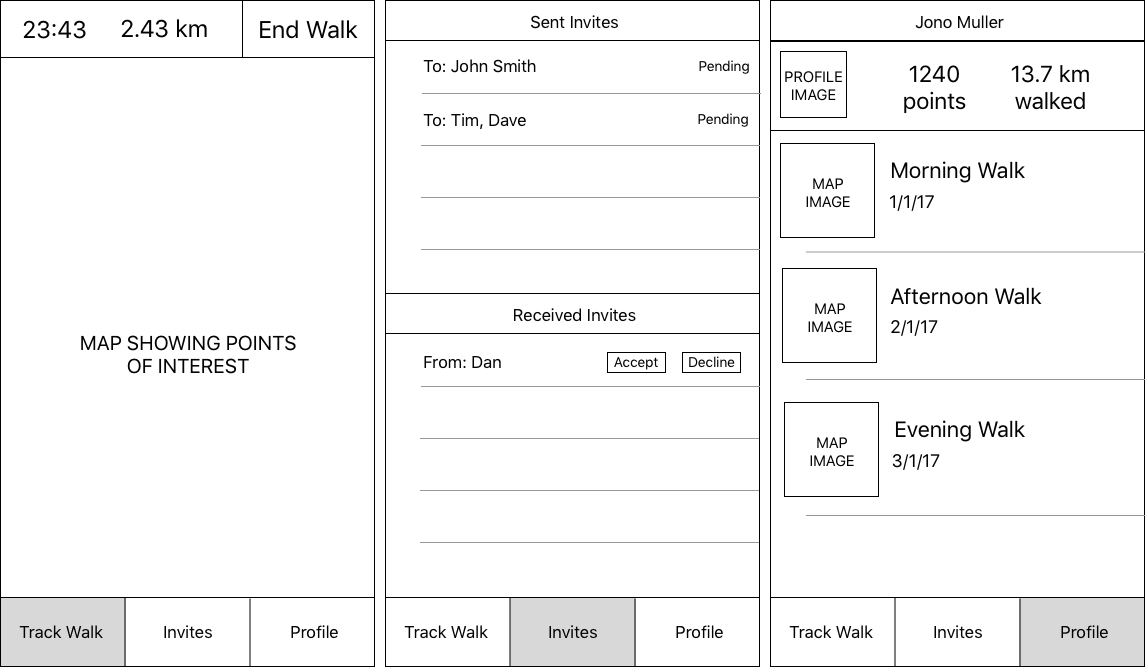
\includegraphics[width=\textwidth]{initial-mockups}
  \caption{Initial mockups of the mobile application, showing how the app is split up into three main sections using the tab bar design.}
  \label{fig:initial-mockups}
\end{figure}

As the design process wore on, I was able to create more detailed mockups utilising more of the resources from the Human Interface Guidelines. I updated the mockups so that each screen of the application contained a navigation bar -- a widely-used UI design pattern in iOS. Setting this as a standard throughout the app provides the user with a constant place where they can navigate between screens of the app and alter content that is displayed on the current screen. I also chose to use collections to display the list of walks on a user's profile instead of the standard tabular method, mainly due to its more visual approach. The updated mockups for the profile view containing collections and the walk detail view showing a navigation bar can be seen in Figure \ref{fig:profile-detail-mockup}.

\begin{figure}[hbt]
  \centering
  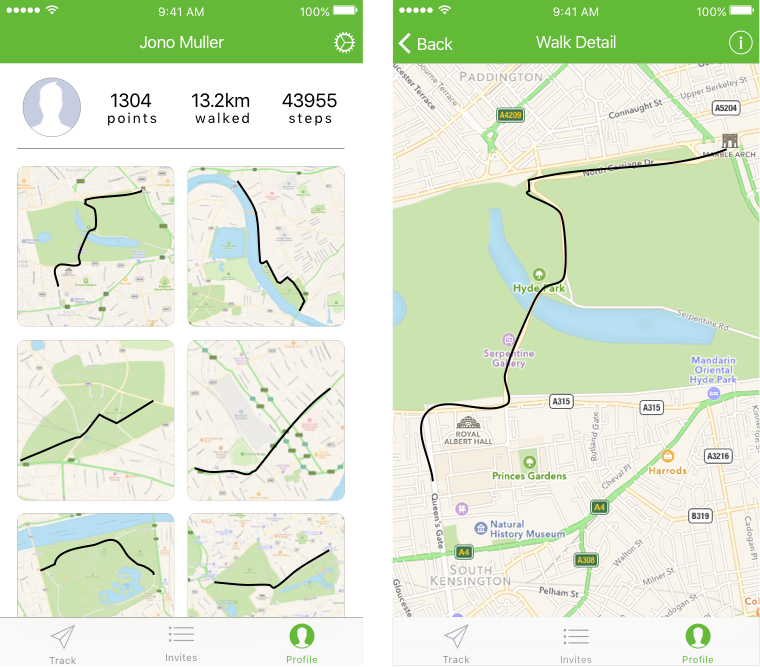
\includegraphics[width=0.9\textwidth]{profile-detail-mockup}
  \caption{Updated mockups of the user profile view (left) that contains a collection of the user's walks, and the walk detail view (right) that is presented when one of the walks from the profile view is selected.}
  \label{fig:profile-detail-mockup}
\end{figure}

Another design element that I chose to use is a segmented control -- a switch containing two or more elements to toggle between different views, normally used to switch between similar content in the same section. Its purpose fits nicely into the invites section of the app, where both sent and received invites need to be displayed but each contains similar information. By using a segmented control, placed in the navigation bar to maximise screen content, users will be able to toggle between viewing their sent and received invites from within the invites tab. The full mockup is displayed in Figure \ref{fig:invites-mockup}.

\begin{figure}[hbt]
  \centering
  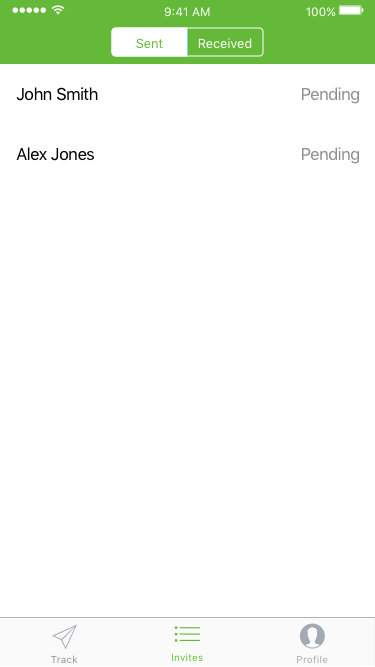
\includegraphics[width=0.45\textwidth]{invites-mockup}
  \caption{Redesigned mockup of the invites section of the application, using a segmented control in the navigation bar to switch between viewing sent and received invites.}
  \label{fig:invites-mockup}
\end{figure}

% login, register mockups
% updated track walk mockups
% summary

\subsection{Model-View-Controller Design Pattern}

An encouraged design pattern to use when creating a mobile application, namely an iOS app, is the Model-View-Controller (MVC) pattern. When following this pattern, objects in an application are split into three layers. Relating to this project, the three layers will be used as follows:

\begin{itemize}
  \item \textbf{Model} stores the data within the application and specifies the logic that alters that data. For this project the model will contain data relating to user information, tracked walk details and invites.
  
  \item \textbf{View} specifies objects that are visible to the user. They can either be used directly from Apple's UIKit framework or customised and reused as needed. The main view objects that are used for this project include a \texttt{MKMapView} which displays a map on screen and a \texttt{UITableView}, useful for displaying an indefinite list of data such as a list of invites.
  
  \item \textbf{Controller} is a medium between the other two layers. It deals with updating the \textbf{Model} based on changes from the \textbf{View} and vice versa. The UIKit framework provides default classes to handle this layer, such as a \texttt{UITableViewController} class that updates a \texttt{UITableView}. A diagram showing how the three layers link together in the project can be seen in Figure \ref{fig:mvc-diagram}.
\end{itemize}

\begin{figure}[hbt]
  \centering
  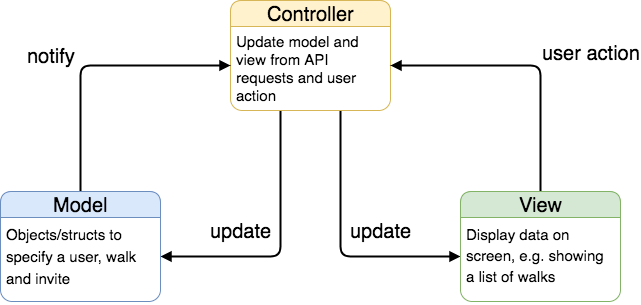
\includegraphics[width=0.8\textwidth]{mvc-diagram}
  \caption{How the Model-View-Controller design pattern links together for this application}
  \label{fig:mvc-diagram}
\end{figure}


% mvc
% tab-bar
% human interface guidelines

\section{API Design}

% REST model, specific endpoints, etc.

Given that the API dealt primarily with JSON because of its easy connectivity with Node.js and MongoDB, responses were returned in JSON. Each response contained a success boolean as one of the values in JSON, determining whether the request was successful or not. HTTP error codes were used to determine the nature of a response as well, but the success flag was useful for error checking within the API.

The following section discusses how the structure of the API is organised as well as how the data was split up in the database.

% add image of how api links to app?

\subsection{Database Models}

% types of models – user, walk, invite, etc.

The data that needed to be stored in the database was split into multiple tables, or collections as they are called in MongoDB, to organise the data effectively. The full UML diagram showing each table's fields and how they link together can be seen in Figure \ref{fig:db-models}. A description of each of the four main tables is as follows:

\begin{itemize}
  \item \textbf{User} stores information about a user, created when they register. It contains cumulative values for the user's score, how far they have walked and how many steps they have taken. It also stores a user's device token, which is used to send a notification to a user's phone when inviting someone to go on a walk.

  \item \textbf{Invite} contains details of an invite sent from one user to one or more other users. Each user in the list of invite recipients contains a boolean flag to indicate whether that user has accepted the invite.

  \item \textbf{Achievement} is a fairly basic collection that stores the type of achievement that was gained from tracking a walk as well as how many points were gained from that achievement. The gamification and achievement aspect of the project is discussed in more detail in Section \ref{subsection:gamification}.
 
  \item \textbf{Walk} stores the details and representation of a walk, given a list of coordinates. It contains a reference to which user(s) tracked the walk, along with what achievements were gained.
\end{itemize}

% add required fields
% write description about each one?

\begin{figure}[hbt]
  \centering
  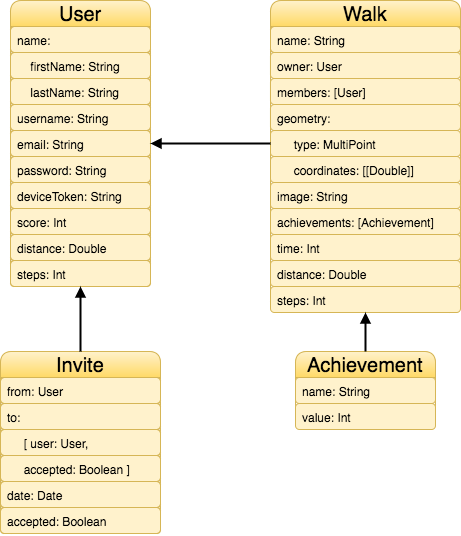
\includegraphics[width=0.7\textwidth]{db-models}
  \caption{Diagram of the different database models used in the project. Arrows indicate where a field in a table references another table.}
  \label{fig:db-models}
\end{figure}

\subsection{Endpoint Structure}

The REST architectural style dictates that each element in the web service uniquely identifies one resource. Based on this, I chose to create a number of endpoints that each provided access to a resource on the server. An endpoint is a reference to a uniform resource indicator (URI) that exposes a resource on the server. These endpoints were grouped into similar categories, where each category is known as a route, to provide clarity to the client. For example, all endpoints that update user information are grouped under the \texttt{/users/} route, with specific user endpoints a subpath of this route. The diagram representation of all of the routes used for the API is shown in Figure \ref{fig:api-routes}.

\begin{figure}[hbt]
  \centering
  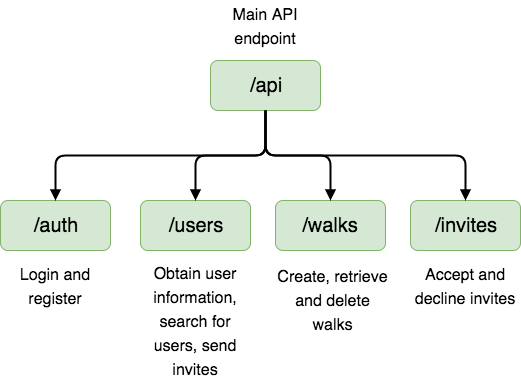
\includegraphics[width=0.7\textwidth]{api-routes}
  \caption{Diagram of each of the routes designed for the API. Each route contains a description of what endpoints exist within that route.}
  \label{fig:api-routes}
\end{figure}

Each endpoint in the API followed the CRUD functions -- standing for Create, Read, Update and Delete. These functions are used to define what operation is being performed when changing data in the database. These functions map to HTTP methods very well, which can then be used in each endpoint to clearly state what operation is used. For example, an endpoint that deletes certain data from the database should adopt the \textit{Delete} function of CRUD and therefore also use the DELETE HTTP method.
 



